\documentclass[10pt]{article}
\usepackage[utf8]{inputenc}
\usepackage{parskip}
\usepackage[margin = 1in]{geometry}
\usepackage{xcolor}
\usepackage[colorlinks = true,linkcolor = blue, urlcolor  = blue,citecolor = blue,anchorcolor = blue]{hyperref}
\usepackage{framed}
\usepackage{apacite}
\usepackage[authoryear,sort]{natbib}
\usepackage{amsmath}
\usepackage{amssymb}
\bibliographystyle{apalike}
\newcommand{\E}{\textrm{E}}
%\renewcommand*{\theenumi}{\thesection.\arabic{enumi}}
\renewcommand{\P}{\text{P}}
\usepackage{tikz}
\usetikzlibrary{arrows,shapes.arrows,positioning,shapes,patterns,calc}

\begin{document}

\begin{Large} 
Info 6751. Fall 2022. Problem Set 10. Due on Canvas by 5pm on 7 Nov.
\end{Large}
\hline \vskip .1in

Note: There have been a lot of assignments lately. This problem set is intentionally brief and asks only conceptual questions to check for understanding---there is no coding nor any math. If you have been tracking things in class, I anticipate you can complete this problem set very quickly.

\section*{Principal stratification (50 points)}

You are examining the causal effect of motherhood ($A = 1$ if any children, $A = 0$ if no children) on hourly wages $Y$.\footnote{This question is widely studied in sociology. See for example Budig, M. J., \& England, P. (2001). \href{https://www.jstor.org/stable/2657415}{\blue{The wage penalty for motherhood.}} American Sociological Review, 204-225. This literature has contributed substantially to the understanding of gender wage gaps as partially generated by the disparate impacts of parenthood on the wages of men and women. To my knowledge, this topic has not been studied from a principal stratification perspective.} But you note that hourly wages $Y$ are only defined for those who are employed ($M = 1$); for those who are not employed, $(\text{Hourly Wage}) = \frac{\text{Pay}}{\text{Hours}} = \frac{0}{0}$ which is nonsensical! Further, unobservable traits $U$ are likely to affect both employment and hourly wages.

In this problem set, we will take motherhood $A$ to be exchangeable: there is no backdoor path $A\leftarrow U \rightarrow Y$. If you would like, you can imagine that we are working with a highly-specific population subgroup, such as married, non-Hispanic white women age 30 with a 4-year college degree who were employed at age 29 as high school teachers. Within this population subgroup, we might believe that motherhood is assigned exchangeably with respect to the potential outcomes.

\begin{center}
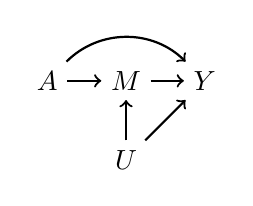
\begin{tikzpicture}
    \node (a) at (0,0) {$A$};
    \node (u) at (1,-1) {$U$};
    \node (m) at (1,0) {$M$};
    \node (y) at (2,0) {$Y$};
    \draw[->, thick] (a) to[bend left = 45] (y);
    \draw[->, thick] (a) -- (m);
    \draw[->, thick] (m) -- (y);
    \draw[->, thick] (u) -- (m);
    \draw[->, thick] (u) -- (y);
\end{tikzpicture}
\end{center}

\begin{enumerate}
\item (8 points) Many researchers restrict to the employed ($M = 1$). Why is this a problem?
\item (16 points) Define each of the following principal strata in words
\begin{itemize}
\item Stratum $S = 1$: All $i$ such that $M_i^1 = M_i^0 = 1$
\item Stratum $S = 2$: All $i$ such that $M_i^1 = M_i^0 = 0$
\item Stratum $S = 3$: All $i$ such that $M_i^1 = 0$ and $M_i^0 = 1$
\item Stratum $S = 4$: All $i$ such that $M_i^1 = 1$ and $M_i^0 = 0$
\end{itemize}
\item (8 points) In which strat(um/a) is the causal effect of motherhood on hourly wages well-defined?
\item (6 points) Is it possible to measure $S$ directly? Why or why not?
\item (6 points) Is $S$ a pre-treatment variable or a post-treatment variable?
\item (6 points) Suppose we assume monotonicity: motherhood might have no effect on employment or reduce employment, but it never causes a woman to become employed. Which stratum is empty under this assumption?
\end{enumerate}

\end{document}

